%
%  untitled
%
%  Created by Ryan Baumann on 2010-10-29.
%  Copyright (c) 2010 __MyCompanyName__. All rights reserved.
%
\documentclass[]{article}

% Use utf-8 encoding for foreign characters
\usepackage[utf8]{inputenc}

% Setup for fullpage use
\usepackage{fullpage}

% Uncomment some of the following if you use the features
%
% Running Headers and footers
%\usepackage{fancyhdr}

% Multipart figures
%\usepackage{subfigure}

% More symbols
%\usepackage{amsmath}
%\usepackage{amssymb}
%\usepackage{latexsym}

% Surround parts of graphics with box
\usepackage{boxedminipage}

% Package for including code in the document
\usepackage{listings}

% If you want to generate a toc for each chapter (use with book)
\usepackage{minitoc}

% This is now the recommended way for checking for PDFLaTeX:
\usepackage{ifpdf}

\usepackage{hyperref}
\hypersetup{
colorlinks = false,
pdfborder = 0 0 0,
pdftitle = {The Son of Suda On-Line},
plainpages = false,
}

\usepackage{attrib}
\usepackage{wrapfig}
\usepackage{subfig}

\usepackage{natbib}
\bibpunct{(}{)}{;}{a}{}{, }
% \usepackage{inlinebib}

%\newif\ifpdf
%\ifx\pdfoutput\undefined
%\pdffalse % we are not running PDFLaTeX
%\else
%\pdfoutput=1 % we are running PDFLaTeX
%\pdftrue
%\fi

\ifpdf
\usepackage[pdftex]{graphicx}
\else
\usepackage{graphicx}
\fi

\usepackage{fontspec,xunicode}
%\setmainfont[ItalicFont={Baskerville-Italic}]{Cardo}
\setmainfont{Adobe Garamond Pro}
\setmonofont[Scale=0.8]{Lucida Grande}

\title{The Son of Suda On-Line}
\author{Ryan Baumann}

\date{}

\begin{document}

\ifpdf
\DeclareGraphicsExtensions{.pdf, .jpg, .tif}
\else
\DeclareGraphicsExtensions{.eps, .jpg}
\fi

\maketitle

\section*{Introduction}

Integrating Digital Papyrology (IDP) is a joint project among a number of institutions aimed at improving and combining the relationships between three digital papyrological resources: the Duke Databank of Documentary Papyri (DDbDP), the Heidelberger Gesamtverzeichnis der griechischen Papyrusurkunden \"{A}gyptens (HGV), and the Advanced Papyrological Information System (APIS). Started in 1983, the DDbDP digitally collects a number of transcriptions of ancient documentary papyri from print editions. HGV and APIS, meanwhile, collect metadata (findspots, dates, etc.) and images of much of the same material. The benefits of unifying these data sources should be obvious, and in 2007 the Scholarly Communications Division of the Andrew W. Mellon Foundation funded a project, “Integrating Digital Papyrology,” to do just that. Over the years the DDbDP has undergone a number of transitions, and this project also supported its transition from an idiosyncratic SGML encoding to standards-based EpiDoc\footnote{\url{http://epidoc.sourceforge.net/}} XML markup. In addition the grant provided funding to improve and finish the first generation of a tool for searching and browsing the unified collection of materials, called the Papyrological Navigator (or PN). At the conclusion of the IDP grant, Mellon funded a second phase of the project (called IDP2) with the following goals:\footnote{\url{http://idp.atlantides.org/trac/idp/wiki/BackgroundAndFunding}}
\begin{quote}
  \begin{enumerate}
    \item Improve operability of the PN search interface on the merged and mapped data from the DDbDP, HGV, and APIS.
    \item Facilitate third-party use of the data and tools.
    \item Create a version controlled, transparent and fully audited, multi-author, web-based, real-time, tagless, editing environment, which — in tandem with a new editorial infrastructure — will allow the entire community of papyrologists to take control of the process of populating these communal assets with data.
  \end{enumerate}
\end{quote}The environment described in the last item, inspired by the Suda On-Line,\footnote{The Suda On-Line (\url{http://www.stoa.org/sol/}) is a project aimed at collaborative translation of the massive 10th century Byzantine encyclopedia known as the \emph{Suda}.} was named the Son of Suda On-Line (SoSOL). Though it takes its name and inspiration from SOL, SoSOL was written from the ground up to incorporate new technologies, address project-specific problems, and move toward more open data and tooling \citep{background, sosin}. This article aims at not only a description of the resulting software, but also of the challenges encountered and solutions chosen in its formulation, to encourage broader adoption or discussion of both.

\section*{The Son of Suda On-Line}

Though collaborative online editing environments such as Wikipedia have the advantage of allowing anyone to contribute, many question the scholarly integrity of resources which can be edited by anyone unvetted. The Suda On-Line, which actually predated the existence of Wikipedia by two years, addressed this problem by marking submitted translations with their level of editorial vetting \citep{finkel}. This combination of openness to contribution with strong editorial control was the guiding principle in the design of the Son of Suda On-Line.

However, even more than SOL, the papyrological projects encompassed in Integrating Digital Papyrology value the scholarly integrity of data published under their aegis. Thus, SoSOL attempts to digitally replicate the scholarly mechanisms of peer review these projects would normally enforce. This results in somewhat of an inversion of where and how editorial control is exerted in comparison with SOL. While SOL users are authorized by editors during registration and are assigned work or must request a specific entry \citep{mahoney}, in SoSOL users are not screened and at present work on whatever they feel needs emendation or inclusion in the corpus. However, this distinction in the assignment of work may just arise naturally from the differing natures of the texts involved; whereas the Suda—while large—is a bounded unit of work, the papyri do not yet show signs of halting their expanding numbers in transcriptions and publications.

Standing in starker contrast is how submissions which have not received editorial oversight are handled: in SOL, they are immediately publicly searchable and accessible but marked as “draft”; in SoSOL, submissions undergo review and voting by an editorial board before publication as “canonical” and being made available for searching in the Papyrological Navigator. This may seem restrictive, or even contradictory to claims of openness. It is indeed the former, but only inasmuch as the editorial boards are controlling the quality of what they are willing to put their names to in the tradition of peer review. The latter requires some discussion.

\subsection*{Data and Openness}

\begin{quote}
“We no longer see IDP as representing at any given moment a synthesis of fixed data sources directed by a central management; rather, we see it as a constantly changing set of fully open data sources governed by the scholarly community and maintained by all active scholars who care to participate. One might go so far as to say that we see this nexus of papyrological resources as ceasing to be “projects” and turning instead into a community.”
\end{quote}\attrib{\citealt{bagnall}}

What do we mean here by “fully open”?

On one level, it is the terms under which data is published.
Though asserting any sort of copyright on the 2,000-year-old texts themselves is perhaps nonsensical (at least in the US\footnote{See \emph{Bridgeman Art Library v. Corel Corp.}}), the complete set of IDP XML files are published with a Creative Commons Attribution 3.0 License,\footnote{\url{http://creativecommons.org/licenses/by/3.0/}} explicitly permitting the typical varieties of scholarly reuse and citation anticipated for the data. (Atypical and unanticipated forms of reuse would be even more exciting.)

On another level, it is the \emph{manner} in which data is published. For collaborative online projects, this is usually a challenge. If the data is constantly changing, how do you publish it in any traditional sense? Perhaps even more challenging is this: how do you publish the changes themselves, both retroactively and proactively?

By retroactively, we mean that the revision history of the data up to the present may itself be important; by proactively we mean that if a user has already obtained the complete revision history at some point in time, it is better to allow them to simply download the changes since that point. Many online collaborative environments, such as MediaWiki and the original SOL, store all changes in a database system. This usually makes distribution of the complete revision history, particularly proactive distribution, extremely difficult. As an example, the English Wikipedia was unable to distribute its complete dataset for several years, and was only most recently able to dump its revision history in January 2010, with no successful exports since.\footnote{\url{http://en.wikipedia.org/w/index.php?title=Wikipedia:Database_download&oldid=393163797\#Latest_complete_dump_of_English_Wikipedia}} Even if they were able to do so, the only mechanism for updating such a data dump is to download the entire several-hundred-gigabyte file each time.

\subsection*{Next-Generation Version Control}

We felt that the best way to approach this problem was to use a \emph{Revision Control System} as the backend for the data itself, instead of a traditional database. Though there are many well-established centralized systems such as CVS and Subversion, in recent years there has been an explosion in the popularity of \emph{distributed} version control systems (DVCSs). Typically this means there is no “central” server except by social convention; all copies of the repository are in a sense equal and can share changes with one another. This allows for a variety of workflow styles, and has a number of other important impacts.

One of the most popular distributed version control systems is Git, initially developed by Linus Torvalds for managing the Linux kernel software project. Due to its broad acceptance, design choices, and proven performance on a number of large projects, it is the backend we selected for data in SoSOL. The SoSOL codebase itself was also managed with Git from the beginning, and is available online.\footnote{\url{http://sourceforge.net/projects/sosol/}}

As a result of using a DVCS for the data backend, it is possible to use Git not only to retrieve both the complete revision history of the IDP data as managed by SoSOL\footnote{\url{http://halsted.vis.uky.edu/gitweb?p=idp.data.git}} (retroactive publication), but also easily update your copy of the repository as changes are published (proactive publication). Due to the distributed nature of Git, the concepts of branching development and merging changes have been integrated into its design, making it easy to keep your copy of the data up-to-date even if you have made your own modifications. (After all, if anyone can pull changes from any other copy of the repository, merging needs to be fast and easy.) The long-running version of this behavior of splitting off your own modifications is known in the open source world as “forking”. Git reduces the overhead of both forking a project, as well as of contributing your forked changes back.

That a DVCS makes these things trivial also represents a significant decision in the design of SoSOL: for the “canonical” data repository it interacts with, it does not need to care about any external mechanisms or workflows used to introduce changes. SoSOL only needs to keep track of changes within its domain; it is merely a front-end and social infrastructure for easing and managing contributions. When a user edits data in SoSOL, it is forked from the main repository to allow them to do their work without interruption. They then submit their changes for editorial review, and when they pass muster they are merged back into the canonical repository. However, the repository may be updated by any external process in the interim, typically without drastically impacting the work that must be done to perform the merge.

Thus the fact that IDP now uses Git for its public data repository, in combination with the license the data is distributed under, represents the complete realization of “a constantly changing set of fully open data sources governed by the scholarly community and maintained by all active scholars who care to participate.” For us, “participate” in fact has two senses: participating within \emph{our} system (that is, participating in our editorial review process), or participating in any enterprise you choose with the complete dataset which we make freely available.

\section*{Implementation}

The Son of Suda On-Line tool itself is written in Ruby using the popular Rails web framework. Instead of the mainline Ruby interpreter written in C (usually referred to as Matz's Ruby Interpreter, or MRI, after the language's creator), we use a Java implementation called JRuby. Though this was initially done to enable deployment of SoSOL in any Java Servlet Container such as Tomcat, SoSOL has come to use a number of Java libraries (particularly for interacting with XML data), facilitated by JRuby's tight Java integration.

\subsection*{Git Internals}

Some discussion of how Git works and internally represents version history is perhaps necessary to illustrate how its design enables and informs other design decisions in SoSOL. In Git, the version history of a project is encoded as a directed graph of three kinds of internal objects, all of which are identified by the unique SHA-1 hash of the object's content. These objects form the “nodes” in Git's graph, their contents contain the directional arrows linking them together.

The simplest instance of version history (in Git, and conceptually) is a single piece of content with one version. Bare content is the “blob” object in Git, and has no additional metadata associated with it — these can be thought of as leaf nodes in the graph (that is, nodes which do not point to other nodes).

However, having just one file is not very useful for most projects. Git organizes and collects multiple blob objects into a file structure using tree objects. These tree objects are simple plaintext files which list identifying hashes with their filenames. Each tree object represents a single directory; for subdirectories, trees can point to other tree objects in addition to blobs, as in Figure \ref{gittree}.

Revisions in Git are stored as commit objects. These point to a single tree, and contain metadata about the commit (such as author, time, commit message) as well as pointers to one or more parent commit objects. Thus, a simple merge would have two parent commits, while a branch or fork would be two different commits pointing to the same commit. The fact that all of this history is stored as a connected graph is what allows the Git system itself to examine things such as where a fork occurred when attempting to merge concurrent changes, and intelligently make the right decision based on the chosen merge strategy.

Let's walk through a simple linear commit history to illustrate things, winding up with the graph shown in Figure \ref{gitcommit}:

\begin{figure}[h]
  \centering
  \subfloat[A tree graph in Git]{\label{gittree}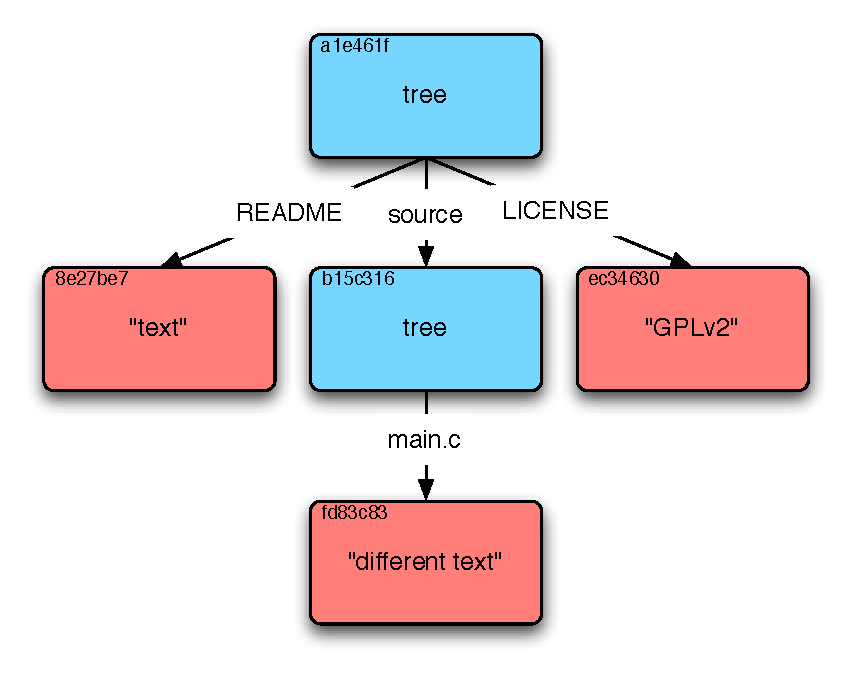
\includegraphics[height=2in]{images/tree.pdf}}
  \qquad
  \subfloat[A series of commits in Git]{\label{gitcommit}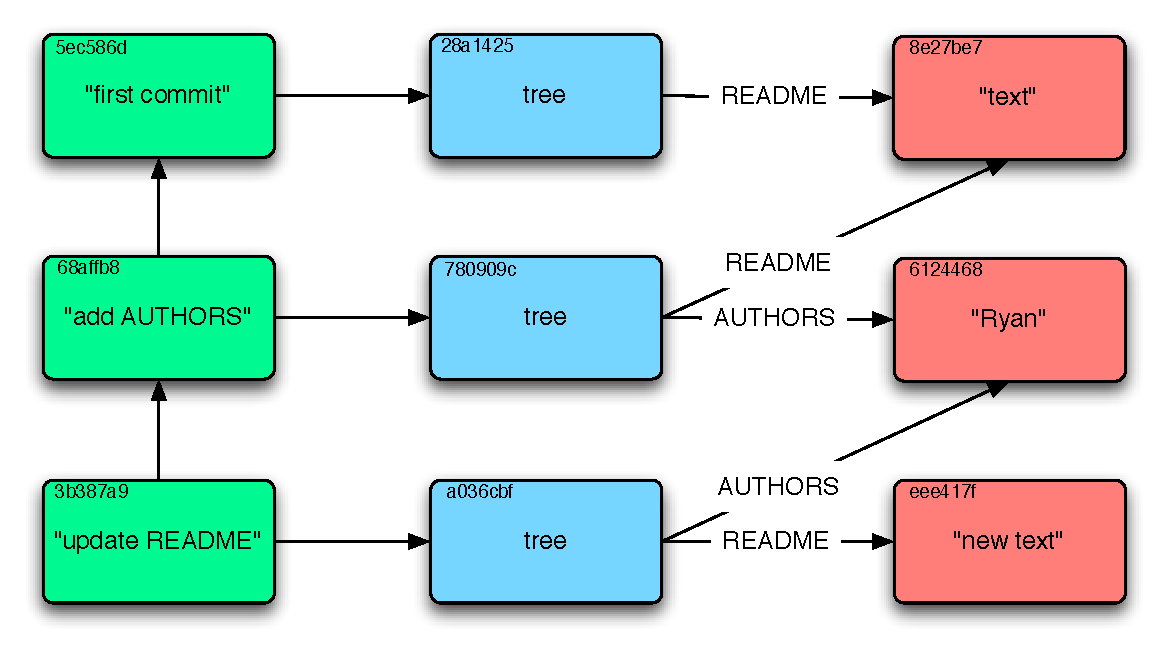
\includegraphics[height=2in]{images/commits.pdf}}
  \caption[]%
    {Visualizations of Git's internal graph structure. Red squares are blobs, blue are trees, green are commits. Text in the top-left corner is the object's truncated hash.}
\end{figure}

\begin{enumerate}
\item We start our project with just a \texttt{README} file containing the string “text”. Since we want to record this momentous occasion, we commit the state of our repository with the commit message “first commit”. This commit points to the hash of the tree, which contains the hash of our \texttt{README}.
\item Since this project is sure to be our magnum opus, we quickly decide we want to immortalize contributors by crediting them in an \texttt{AUTHORS} file. We write this out and hastily make a new commit to add it. Since the \texttt{README} is unchanged, the same object from before is reused. However, because we have added a new file, the tree has changed, so a new tree object is made for the commit to point to.
\item Later, the mood strikes us to update the \texttt{README} so we do so and make a new commit. Again, a new blob object is constructed for the new content, although this time the \texttt{AUTHORS} blob is able to be reused because we didn't modify it.
\end{enumerate}
\subsection*{Data Sources, Publications, and Workflow}

As outlined in the introduction, IDP represents the synthesis of a variety of papyrological projects managed by different institutions. This has informed SoSOL's design in how it interacts with and models these disparate data sources.

\begin{figure}[h]
  \centering
  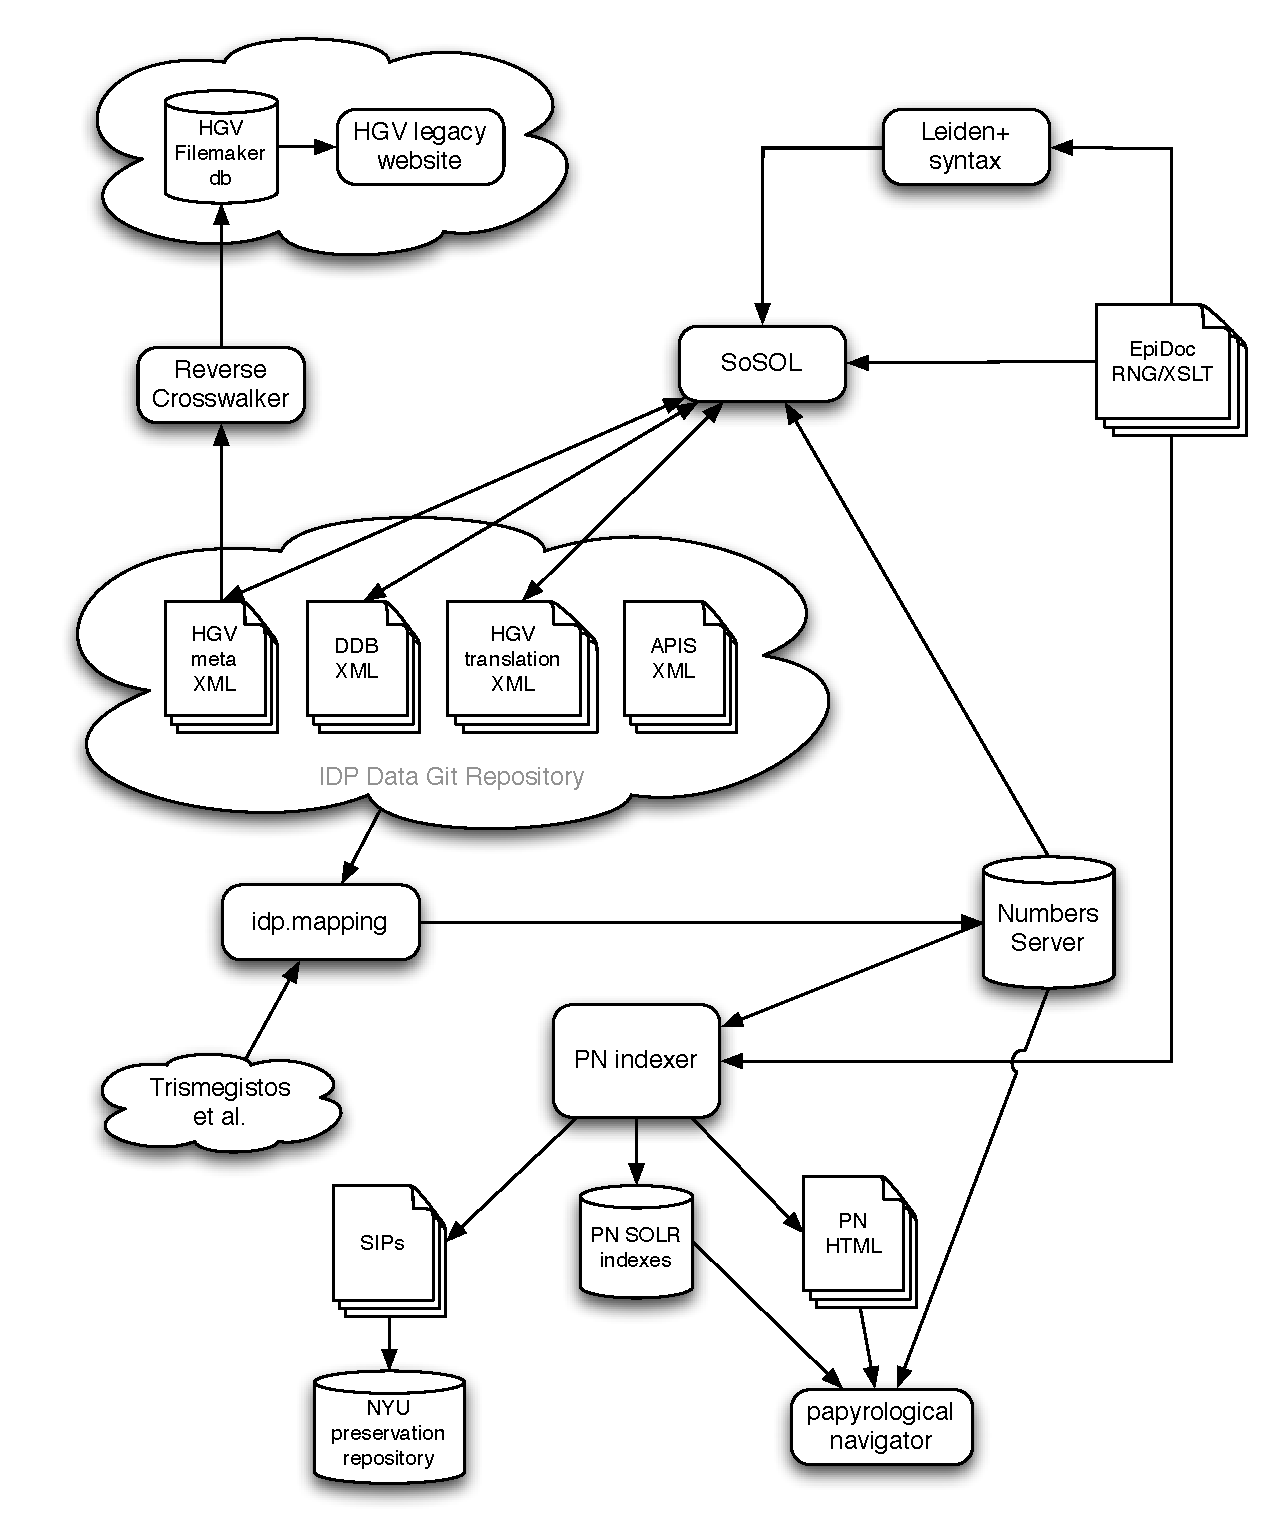
\includegraphics[width=6in]{images/TopLevelDataFlow4Proposal-HAC.pdf}
  \caption{Software components and data flow at the conclusion of IDP2\label{dataflow}}
\end{figure}

\subsection*{Alternative Syntax for XML Editing}

\begin{figure}[ht]
    \begin{verbatim}
[ἔτους α (?) Αὐτοκράτορος]   ̣  ̣[  ̣]  ̣  ̣του 
[- ca.12 -] Σεβαστοῦ 
[εἴργ(ασται) ὑ(πὲρ) χω(ματικῶν) ἔ]ργ(ων) τοῦ αὐτοῦ̣ πρώτου (ἔτους) 
[ -ca.?- ] κ κϛ ἐ[ν] τῇ Ἐπα -
[γαθιαν]ῇ διώ(ρυγι) Βακχιά(δος) 
[ -ca.?- ] Πατκ(όννεως) τοῦ Θεαγένους 
[  ̣  ̣  ̣  ̣  ̣  ̣] μη(τρὸς) Ταύρεως 
[ -ca.?- ] (hand 2) σεση(μείωμαι)
    \end{verbatim}
    \caption{Typical print transcription following Leiden conventions (P.Sijp., 41a)\label{leiden}}
\end{figure}\nocite{psijp}

\begin{figure}[h]
    \begin{verbatim}
1. [ἔτους] [<#α=1#> (?)] [Αὐτοκράτορος] .2[.1].2του
2. [ca.12] Σεβαστοῦ
3. [(εἴργ(ασται)) (ὑ(πὲρ) χω(ματικῶν))] ([ἔ]ργ(ων)) τοῦ αὐτοῦ̣ πρώτου ((ἔτους))
4. [.?] <#κ=20#>  <#κϛ=26#> ἐ[ν] τῇ Ἐπα
5.- [γαθιαν]ῇ (διώ(ρυγι)) (Βακχιά(δος))
6. [.?] (Πατκ(όννεως)) τοῦ Θεαγένους
7. [ca.6] (μη(τρὸς)) Ταύρεως
8. [.?] $m2 (σεση(μείωμαι))
    \end{verbatim}
    \caption{Leiden+ representation of the same text\label{leidenp}}
\end{figure}

\begin{figure}[hb]
  \begin{verbatim}
<div xml:lang="grc" type="edition" xml:space="preserve">
  <ab>
    <lb n="1"/><supplied reason="lost">ἔτους</supplied> <supplied
      reason="lost" cert="low"><num value="1">α</num> </supplied> <supplied
      reason="lost">Αὐτοκράτορος</supplied> <gap reason="illegible" quantity="2"
      unit="character"/><gap reason="lost" quantity="1" unit="character"/><gap
      reason="illegible" quantity="2" unit="character"/>του
    <lb n="2"/><gap reason="lost" quantity="12" unit="character"
      precision="low"/> Σεβαστοῦ
    <lb n="3"/><supplied reason="lost"><expan>εἴργ<ex>ασται</ex></expan>
      <expan>ὑ<ex>πὲρ</ex> χω<ex>ματικῶν</ex></expan></supplied>
      <expan><supplied reason="lost">ἔ</supplied>ργ<ex>ων</ex></expan> τοῦ
      αὐτο<unclear>ῦ</unclear> πρώτου <expan><ex>ἔτους</ex></expan>
    <lb n="4"/><gap reason="lost" extent="unknown" unit="character"/> <num
      value="20">κ</num> <num value="26">κϛ</num> ἐ<supplied
      reason="lost">ν</supplied> τῇ Ἐπα
    <lb n="5" type="inWord"/><supplied reason="lost">γαθιαν</supplied>ῇ
      <expan>διώ<ex>ρυγι</ex></expan> <expan>Βακχιά<ex>δος</ex></expan>
    <lb n="6"/><gap reason="lost" extent="unknown" unit="character"/>
      <expan>Πατκ<ex>όννεως</ex></expan> τοῦ Θεαγένους
    <lb n="7"/><gap reason="lost" quantity="6" unit="character"
      precision="low"/> <expan>μη<ex>τρὸς</ex></expan> Ταύρεως
    <lb n="8"/><gap reason="lost" extent="unknown" unit="character"/>
      <handShift new="m2"/><expan>σεση<ex>μείωμαι</ex></expan>
  </ab>
</div>
  \end{verbatim}
  \caption{EpiDoc XML fragment equivalent to the preceding Leiden+\label{epidoc}}
\end{figure}




\section*{Conclusions}

\bibliographystyle{plainnat}
\bibliography{bics-sosol}
\end{document}
